\section{Thiết kế dự án}

\subsection{Tổng quan các chế độ hoạt động}
Hệ thống vận hành với 3 chế độ hoạt động chính:
\begin{enumerate}
    \item \textbf{Chế độ Tự động (\texttt{APP\_MODE\_AUTO})}: Hệ thống tự động chuyển pha đèn giao thông cho Tuyến 1 và Tuyến 2 theo chu kỳ thời gian được cài đặt. Để đảm bảo an toàn thực tế, giữa các lần hoán đổi tuyến ưu tiên luôn có pha đệm an toàn (\textit{All-Red clearance phase}), trong đó cả hai tuyến cùng đỏ trong thời gian $T_{\text{clearance}} = 1\text{s}$ nhằm giải phóng toàn bộ phương tiện đang lưu thông trong giao lộ.
    \item \textbf{Chế độ Bằng tay (\texttt{APP\_MODE\_MANUAL})}: Dành cho trường hợp cảnh sát giao thông hoặc nhân viên điều phối can thiệp trực tiếp vào nút giao. Mỗi lần nhấn Nút 2 (Action), hệ thống sẽ nhảy sang bước kế tiếp trong quy trình tuần tự. Đặc biệt, hệ thống đi qua trạng thái đệm All-Red trước khi cấp quyền ưu tiên cho tuyến tiếp theo, tuyệt đối triệt tiêu nguy cơ hai tuyến cùng xanh.
    \item \textbf{Chế độ Chỉnh thời gian (\texttt{APP\_MODE\_TUNING})}: Cho phép người vận hành điều chỉnh thời lượng sáng của đèn Đỏ, Xanh và Vàng hiển thị trực tiếp trên màn hình LCD. Hệ thống cung cấp cơ chế kiểm soát tự động để đảm bảo thời gian thiết lập luôn thỏa mãn điều kiện logic an toàn trước khi lưu trữ và áp dụng vào chu kỳ tự động.
\end{enumerate}

Ngay sau khi hệ thống được cấp nguồn hoặc reset phần cứng, hệ thống khởi tạo ngoại vi và lập tức tiến vào \textbf{Chế độ Tự động} với trạng thái xuất phát an toàn: Cả hai tuyến cùng bật đèn Đỏ, sau đó kích hoạt pha đầu tiên (Tuyến 1 Đỏ, Tuyến 2 Xanh).

Bảng~\ref{tab:button_mapping} mô tả chi tiết chức năng của các nút nhấn vật lý trong từng chế độ hoạt động:

\begin{table}[H]
\centering
\small
\begin{tabularx}{\textwidth}{|l|c|X|X|X|}
\hline
\textbf{Nút nhấn} & \textbf{Chân STM32} & \textbf{Chế độ Tự động} & \textbf{Chế độ Bằng tay} & \textbf{Chế độ Chỉnh thời gian} \\ \hline
\textbf{Nút 1 (D7)} & PA8 & Chuyển sang Manual & Chuyển sang Tuning & Chuyển về Auto \\ \hline
\textbf{Nút 2 (D8)} & PA9 & Không tác vụ & Chuyển bước (Next Step) & Chuyển trường chỉnh (RED $\rightarrow$ GREEN $\rightarrow$ YELLOW) \\ \hline
\textbf{Nút 3 (D9)} & PC7 & Không tác vụ & Không tác vụ & Giảm giá trị (Decrease) \\ \hline
\textbf{Nút 4 (D10)} & PB6 & Không tác vụ & Không tác vụ & Tăng giá trị (Increase) \\ \hline
\textbf{Nút USER} & PC13 & Phục vụ mở rộng & Phục vụ mở rộng & Phục vụ mở rộng \\ \hline
\end{tabularx}
\caption{Chức năng của các nút nhấn theo từng chế độ hoạt động}
\label{tab:button_mapping}
\end{table}

\subsection{Máy trạng thái chuyển chế độ}
Bộ quản lý chế độ (\texttt{fsm\_mode\_manager}) đóng vai trò là FSM mức cao nhất trong hệ thống, điều phối việc chuyển đổi giữa 3 chế độ lớn thông qua Nút 1 (\texttt{FSM\_BUTTON\_MODE}).

\begin{figure}[H]
\centering
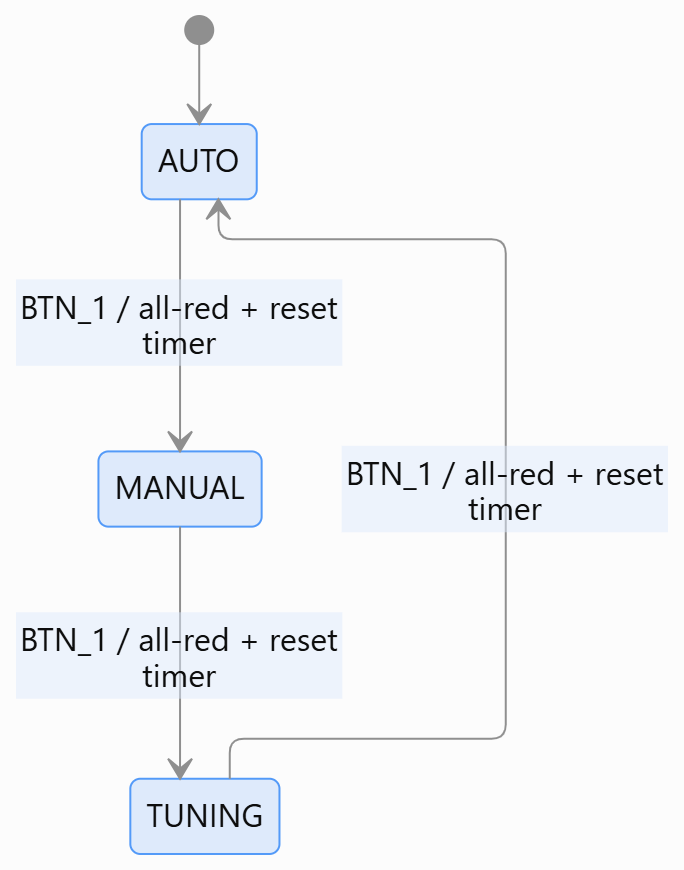
\includegraphics[width=0.75\textwidth]{graphics/fsm_mode_manager.png}
\caption{Sơ đồ máy trạng thái chuyển đổi giữa các chế độ lớn}
\label{fig:fsm_mode_manager}
\end{figure}

Sơ đồ chuyển trạng thái của bộ quản lý chế độ được tổng hợp ở Bảng~\ref{tab:mode_transitions}:

\begin{table}[H]
\centering
\small
\begin{tabularx}{\textwidth}{|l|l|l|X|}
\hline
\textbf{Chế độ hiện tại} & \textbf{Sự kiện kích hoạt} & \textbf{Chế độ kế tiếp} & \textbf{Hành động an toàn khi chuyển đổi} \\ \hline
\texttt{APP\_MODE\_AUTO} & Nhấn Nút 1 (\texttt{BTN\_1}) & \texttt{APP\_MODE\_MANUAL} & Cưỡng bức cả 2 tuyến về Đỏ (All-Red), reset Phase Timer, khởi tạo trạng thái ban đầu của Manual FSM. \\ \hline
\texttt{APP\_MODE\_MANUAL} & Nhấn Nút 1 (\texttt{BTN\_1}) & \texttt{APP\_MODE\_TUNING} & Cưỡng bức cả 2 tuyến về Đỏ (All-Red), reset Phase Timer, khởi tạo màn hình LCD cho Tuning FSM. \\ \hline
\texttt{APP\_MODE\_TUNING} & Nhấn Nút 1 (\texttt{BTN\_1}) & \texttt{APP\_MODE\_AUTO} & Chuẩn hóa ràng buộc thời gian ($T_{\text{Đỏ}} \ge T_{\text{Xanh}} + T_{\text{Vàng}} + 2$), cưỡng bức 2 tuyến về Đỏ, nạp cấu hình thời gian mới và khởi chạy Auto FSM. \\ \hline
\end{tabularx}
\caption{Bảng chuyển trạng thái giữa các chế độ lớn}
\label{tab:mode_transitions}
\end{table}

\subsection{Phân tích chuyển đổi giữa các chế độ lớn}
Phần chuyển đổi chế độ là mắt xích quan trọng nhất quyết định độ an toàn của hệ thống nhúng trong thực tế. Bất kỳ sự chuyển trạng thái đột ngột nào không qua pha trung gian đều có thể dẫn đến việc các phương tiện đang di chuyển ở tốc độ cao gặp đèn chuyển pha đột ngột hoặc nguy cơ hai tuyến cùng xanh. Nhóm đã hiện thực giải thuật chuyển đổi an toàn thông qua hàm tập trung \texttt{enter\_mode(next\_mode)}:

\subsubsection{Từ chế độ tự động sang chế độ bằng tay}
\begin{itemize}
    \item \textbf{Trạng thái đèn ngay sau khi chuyển}: Dù chế độ tự động đang ở bất kỳ pha nào (kể cả đang Xanh ở một tuyến), hàm chuyển đổi lập tức gọi \texttt{set\_both\_roads\_red()}, kích hoạt đèn Đỏ trên cả hai tuyến. Chế độ Manual xuất phát từ Bước 0 (\texttt{MAN R1:RD R2:RD}), giữ cả 2 tuyến Đỏ cho đến khi người vận hành chủ động nhấn Nút 2 để cấp quyền di chuyển.
    \item \textbf{Quản lý Task và Timer}: Bộ đếm \texttt{FSM\_PHASE\_TIMER} trong module \texttt{software\_timer} được đặt về 0 để hủy bỏ chu kỳ đếm tự động cũ. FSM Manual được cấp quyền xử lý tín hiệu từ Nút 2.
    \item \textbf{Hiển thị LCD}: Màn hình LCD lập tức xóa nội dung cũ và hiển thị dòng chữ \texttt{"MAN  R1:RD R2:RD"} ở dòng 1. Dòng 2 tiếp tục hiển thị thông số môi trường cập nhật từ DHT20.
    \item \textbf{Tính an toàn}: Loại bỏ hoàn toàn khả năng xung đột đèn khi bàn giao quyền điều khiển từ máy sang người.
\end{itemize}

\subsubsection{Từ chế độ bằng tay sang chế độ chỉnh thời gian}
\begin{itemize}
    \item \textbf{Trạng thái đèn}: Hệ thống tiếp tục duy trì trạng thái All-Red (\texttt{TL\_RED} trên cả hai tuyến) trong suốt thời gian người dùng cấu hình thông số, đảm bảo giao lộ tạm dừng hoặc ở trạng thái an toàn tuyệt đối khi hệ thống đang ở chế độ cài đặt.
    \item \textbf{Xử lý biến và trạng thái}: Con trỏ trường điều chỉnh được gán về mặc định là trường đèn Đỏ (\texttt{TUNE\_RED}). Các giá trị biến toàn cục $g\_red\_time\_s$, $g\_green\_time\_s$, $g\_yellow\_time\_s$ được nạp vào bộ nhớ tạm để chuẩn bị cho thao tác tăng/giảm.
    \item \textbf{Hiển thị LCD}: Dòng 1 LCD hiển thị trường đang chọn cùng giá trị thời gian tính theo giây (ví dụ: \texttt{"SET RED:  030s"}). Dòng 2 hiển thị hướng dẫn thao tác nút nhấn (B2:Next, B3:-, B4:+).
\end{itemize}

\subsubsection{Từ chế độ chỉnh thời gian về chế độ tự động}
\begin{itemize}
    \item \textbf{Kiểm tra tính hợp lệ và chuẩn hóa}: Trước khi chuyển về Auto, hàm \texttt{normalize\_timing()} được triệu gọi tự động nhằm kiểm tra các ràng buộc kỹ thuật:
    \begin{equation}
        \begin{cases}
            T_{\text{GREEN}} \in [3\text{s}, 90\text{s}] \\
            T_{\text{YELLOW}} \in [1\text{s}, 10\text{s}] \\
            T_{\text{RED}} \ge T_{\text{GREEN}} + T_{\text{YELLOW}} + 2 \times T_{\text{clearance}} \\
            T_{\text{RED}} \le 180\text{s}
        \end{cases}
    \end{equation}
    Nếu người dùng vô tình đặt $T_{\text{RED}}$ nhỏ hơn tổng thời gian Xanh + Vàng + đệm an toàn, hệ thống sẽ tự động ép giá trị $T_{\text{RED}}$ lên mức tối thiểu an toàn, ngăn chặn hoàn toàn lỗi logic chu kỳ đèn.
    \item \textbf{Áp dụng thời gian mới vào chu kỳ}: Các giá trị đã chuẩn hóa được nạp chính thức vào chu kỳ của \texttt{fsm\_automatic}. Pha ban đầu được đặt lại là Tuyến 1 Đỏ, Tuyến 2 Xanh, bộ đếm thời gian được nạp lại ứng với giá trị thời gian mới, và hệ thống bắt đầu chu kỳ vận hành tự động trơn tru.
\end{itemize}
